\documentclass[a4paper,10pt]{report}

\advance\textwidth by 6cm
\advance\oddsidemargin by -3cm
\advance\evensidemargin by -3cm

\advance \topmargin -2cm
\advance \textheight 4cm


%opening
\title{Getting Started Guide \\  Bayesian Filtering Library}
\author{Tinne De Laet, Wim Meeussen, Klaas Gadeyne}

\usepackage{amsmath}
\usepackage{subfigure}
\usepackage{graphicx,color,psfrag}
\usepackage{epsfig} 
\usepackage{fancyvrb} 
\usepackage{fancybox} 
\usepackage{verbatim}
\usepackage{keyval}
\usepackage{url}
%\usepackage[]{tex4ht}

%\graphicspath{{figures_src/}}

\begin{document}

\maketitle


% -----------------------------------------------------------
% --- INTRODUCTION ------------------------------------------
% -----------------------------------------------------------


%----------------------------------
\chapter{Introduction to BFL}
%----------------------------------
\section{What is BFL?}
The Bayesian Filtering Library (BFL) has been designed with the
following requirements in mind:
\begin{itemize}
\item [Bayesian] BFL provides a fully Bayesian software framework,
  i.e.~all Bayesian methods fit in the library design. Therefore the
  library does not impose restrictions on the nature of the Random
  Variables nor on the representation of the probability density
  function (analytical, sample based, \dots). The common Bayesian
  background of BFL allows to implement different Bayesian algorithms
  with a maximum of code reuse. Moreover, the performance of these
  algorithms can be compared with a minimum effort.
\item [Open] The Open Source Initiative offers an enormous potential
  for the maximum reuse of code and is ideal to study differences
  between different algorithms or different implementations of a
  particular algorithm. Furthermore open source software is a key
  factor implementing the idea of \emph{reproducible research}. The
  state of the art can only benefit from the availability of the
  source code, in order to reproduce the obtained results and to gain
  better understanding by altering certain chosen values of the
  experiments.
\item [Independent] The first meaning of independent is the
  independence to the numerical and stochastical library. At present,
  there is no \emph{standard} numerical nor stochastical library for
  C++ \ available, there's a wide range of libraries available
  providing the necessary functionality. An estimation library is only
  a part of the whole software infrastructure in order to perform a
  certain task. To avoid ending up with multiple libraries for one
  project, BFL is decoupled possible from one particular
  numerical/stochastical library.

  The second meaning of independent is the independence of BFL of a
  particular application (such as Autonomous Compliant Motion, mobile
  robotics, econometrics, \dots). This means both its interface and
  implementation are decoupled from particular sensors, assumptions,
  algorithms, \dots that are specific to a certain application.
\end{itemize}
Furthermore, BFL is integrated in our robot control software written
in C++ \ and therefore, C++ \ is chosen as programming language.

\section{BFL's History}
BFL was born during the PhD research of Klaas Gadeyne (See
\url{http://people.mech.kuleuven.be/~kgadeyne/}).  Through an analysis
of the general Bayesian framework underneath the above mentioned
Bayesian filters, he designed the state estimation software
framework/library BFL, containing support for different filters (in
particular Sequential Monte Carlo methods and Kalman filters, but also
e.g.~grid based methods) and easily extendible towards other Bayesian
methods. Late 2001, BFL was released as an open source project, and is
since then slowly growing and maturing.

\section{Getting support - the BFL community}
There are different ways to get some help/support:
\begin{itemize}
\item This tutorial!
\item The website
  \url{http://www.orocos.org/bfl} with the
  doxygen documentation of BFL. A symbolic link is included to one of
  the svn copies so you can even browse the source code.
\item Klaas Gadeyne's PhD thesis contains a chapter about BFL's design
  (again, see the website)
\item The mailing list (see
  \url{http://lists.mech.kuleuven.be/mailman/listinfo/bfl/}) for
  questions and discussions.
\end{itemize}







%----------------------------------
\chapter{Tutorial}
\label{chapt:tutorial}
%----------------------------------
\section{How to prepare the tutorial examples}

First you get the source of the tutorial examples. To see the source
code of the examples, you need to get the BFL source:
\begin{itemize}
\item You can download the bfl tarbal, or
\item get BFL from subversion.
\end{itemize}
Both cases are explained in the BFL installation guide on
\url{www.orocos.org/bfl}. After doing this, you will find the example
programs in bfl/examples.


Now you are already set to start the tutorial. However, if you also
want to execute the examples, and seen the numerical results yourself,
you need to choose one of these two options:
\begin{itemize}
\item Compile the BFL source as explained in the installation guide,
  and find the binary examples in bf/build/examples
\item Or you can get the precompiled BFL examples from our aptitude
  server. Therefore you need to:\
\begin{enumerate}
\item First add the following line to your /etc/apt/sources.list:
\begin{verbatim}
  deb http://people.mech.kuleuven.be/~tdelaet/bfl _mydistro_ main
\end{verbatim}
  where \emph{\_mydistro\_} is breezy, dapper, edgy or feisty.
\item Then apt-get the packages:
\begin{verbatim}
  sudo apt-get update
  sudo apt-get install orocos-bfl-examples
\end{verbatim}
Now you find the percompiled BFL examples in /usr/bin/bfl.
\end{enumerate}
\end{itemize}





% -----------------------------------------------------------
% --- KALMAN ------------------------------------------------
% -----------------------------------------------------------

\pagebreak
\section{Your first Kalman filter in 15 minutes}
This section will guide you step-by-step through the implementation of
a Kalman filter with a linear system model and a linear measurement
model. We'll describe all implementation steps completely, but we'll
assume that you have some basic knowledge about Bayesian estimation
theory.

In this first example we use a Kalman filter to estimate the position
of a mobile robot. The mobile robot drives around in an open space
with one wall. In this example, the mobile robot can only drive
forward and backwards, and not turn. Using a distance sensor, the
mobile robot measures its distance to this wall.

\begin{figure}
%\resizebox{12cm}{!}{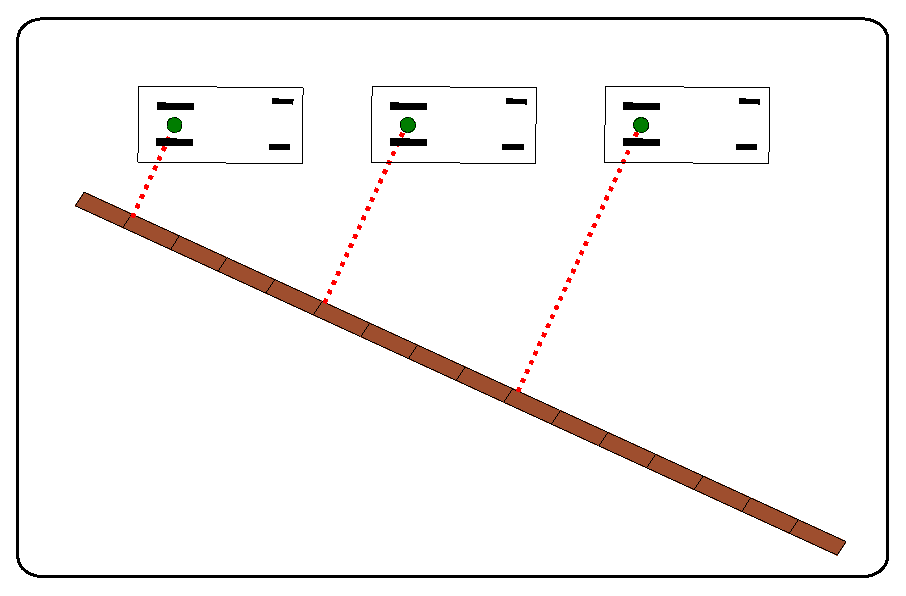
\includegraphics{mobile_robot_simple.eps}}%
\center
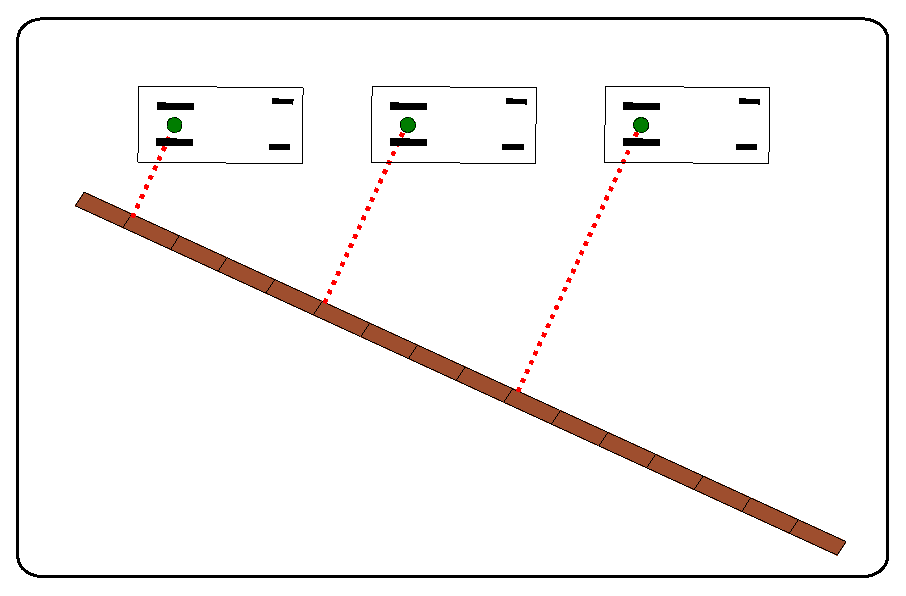
\includegraphics[width=12cm]{mobile_robot_simple.eps}
\caption{Mobile robot}
\label{fig: mobile_robot}
\end{figure}




\subsection{Preparing the .cpp file}
%----------------------------------

In the folder 
\begin{verbatim}
  BFL/tutorial/progs/src/linear_kalman/
\end{verbatim}
you find the source file called 
\begin{verbatim}
  test_linear_kalman.cpp
\end{verbatim}
This file contains the implementation we discuss in this first
example. The beginning of the file contains some C++ overhead, such as
the inclusion of the BFL header files we'll use
\begin{verbatim}
  #include <filter/extendendkalmanfilter.h>
  #include <model/linearanalyticsystemmodel_gaussianuncertainty.h>
  #include <model/linearanalyticmeasurementmodel_gaussianuncertainty.h>
  #include <pdf/linearanalyticsystemmodel_gaussianuncertainty.h>
  #include <pdf/linearanalyticmeasurementmodel_gaussianuncertainty.h>
\end{verbatim}
and the namespaces that we'll use
\begin{verbatim}
  using namespace MatrixWrapper;
  using namespace BFL;
  using namespace std;
\end{verbatim}


\subsection{The linear system model}
%----------------------------------
We'll now build the system model, to make a prediction of the position
of the mobile robot at each time step. The prediction is based on the
velocity of the mobile robot. Because the mobile robot cannot turn,
the prediction of the position is a linear equation. Since the model
is linear, BFL already includes a ready-to-use implementation.

First we build the linear model that calculates the position of the
mobile robot ${x}_{k+1}$, given its previous position ${x}_k$ and its
velocity ${u}_k$ consisting of the translational velocity $v$ and the
rotational velocity $\omega$ (which in this first example is zero).
The linear model is defined by:
\begin{equation}
  {x}_{k+1} = {A} {x}_k +
  {B} {u}_k
\end{equation}
We build the matrices ${A}$ and ${B}$:
\begin{verbatim}
  Matrix A(2,2);
  A(1,1) = 1.0;
  A(1,2) = 0.0;
  A(2,1) = 0.0;
  A(2,2) = 1.0;

  Matrix B(2,2);
  B(1,1) = cos(0.8);
  B(1,2) = 0.0;
  B(2,1) = sin(0.8);
  B(2,2) = 0.0;
\end{verbatim}
and we combine these two matrices in a vector ${AB}$:
\begin{verbatim}
  vector<Matrix> AB(2);
  AB[0] = A;
  AB[1] = B;
\end{verbatim}
Then we create a Gaussian distribution, which is defined by a mean
(Mu) and a covariance (Cov). This Gaussian distribution represents the
uncertainty on the predicted position of the mobile robot. The
mean is chosen to be $0.0$:
\begin{verbatim}
  ColumnVector sysNoise_Mu(2);
  sysNoise_Mu(1) = 0.0;
  sysNoise_Mu(2) = 0.0;
\end{verbatim}
and the covariance is chosen as a diagonal matrix, with $0.01^2$ as the
$\sigma^2$ boundary:
\begin{verbatim}
  SymmetricMatrix sysNoise_Cov(2);
  sysNoise_Cov(1,1) = pow(0.01,2);
  sysNoise_Cov(1,2) = 0.0;
  sysNoise_Cov(2,1) = 0.0;
  sysNoise_Cov(2,2) = pow(0.01,2);
\end{verbatim}
The mean and covariance together define a two dimensional Gaussian
distribution:
\begin{verbatim}
  Gaussian system_Uncertainty(sysNoise_Mu, sysNoise_Cov);
\end{verbatim}
Now we create a linear conditional probability density function (pdf)
which represents the probability of the predicted position given the
current position of the mobile robot. This pdf is defined by the
vector ${AB}$ which represents the linear model, together with the
Gaussian distribution which represents the system model's extra
uncertainty.
\begin{verbatim}
  LinearAnalyticConditionalGaussian sys_pdf(AB, system_Uncertainty);
\end{verbatim}
Finally we create the system model from the system pdf:
\begin{verbatim}
  LinearAnalyticSystemModelGaussianUncertainty sys_model(&sys_pdf);
\end{verbatim}




\subsection{The linear measurement model}
%----------------------------------
We'll now build the measurement model, to correct the prediction of
the position of the mobile robot, based on the distance measurement to
the wall. Since we use a linear measurement model in this example, BFL
already includes a ready-to-use implementation.

First we build the linear model that links the distance measurement to
the position of the mobile robot.
\begin{equation}
  {z}_{k+1} = {H} {x}_{k+1}
\end{equation}
We build the matrix ${H}$:
\begin{verbatim}
  Matrix H(1,2);
  H(1,1) = 0.0;
  H(1,2) = 2.0;
\end{verbatim}
Then we create a Gaussian distribution, which is defined by a mean
(Mu) and a covariance (Cov). This Gaussian distribution represents the
uncertainty on the measured distance to the wall. The mean is $0.0$:
\begin{verbatim}
  ColumnVector measNoise_Mu(1);
  measNoise_Mu(1) = 0.0;
\end{verbatim}
and the covariance is diagonal matrix, with $0.05^2$ as the $\sigma^2$
boundary:
\begin{verbatim}
  SymmetricMatrix measNoise_Cov(1);
  measNoise_Cov(1,1) = pow(0.05,2);
\end{verbatim}
The mean and covariance together define a two dimensional Gaussian
distribution:
\begin{verbatim}
  Gaussian measurement_Uncertainty(measNoise_Mu, measNoise_Cov);
\end{verbatim}

Now we create a linear probability density function (pdf) which
represents the probability of the distance measurement. This pdf is
defined by the matrix ${H}$ which represents the linear model,
together with the Gaussian distribution which represents the
measurement uncertainty.
\begin{verbatim}
  LinearAnalyticConditionalGaussian meas_pdf(H,
measurement_Uncertainty);
\end{verbatim}
Finally we create the measurement model from the measurement pdf:
\begin{verbatim}
  LinearAnalyticMeasurementModelGaussianUncertainty meas_model(&meas_pdf);
\end{verbatim}





\subsection{Prior Distribution}
%----------------------------------
We'll now build the prior distribution representing the initial
estimate and the uncertainty associated with this initial estimate.\\
The prior distribution is a Gaussian distribution with mean
(prior\_Mu) and covariance (prior\_Cov).  The mean is the initial
estimated state:
\begin{verbatim}
  ColumnVector prior_Mu(2);
  prior_Mu(1) = -1.0;
  prior_Mu(2) = 1.0;
\end{verbatim}
and the covariance is a diagonal matrix, with $1.0$ as the $\sigma^2$
boundary:
\begin{verbatim}
  SymmetricMatrix prior_Cov(2);
  prior_Cov(1,1) = 1.0;
  prior_Cov(1,2) = 0.0;
  prior_Cov(2,1) = 0.0;
  prior_Cov(2,2) = 1.0;
\end{verbatim}
The mean and covariance together define a two dimensional Gaussian
distribution:
\begin{verbatim}
  Gaussian prior(prior_Mu, prior_Cov);
\end{verbatim}




\subsection{Construction of the filter}
In this example we want to use a Kalman filter to estimate the unknown
position of the mobile robot. BFL provides the class
ExtendedKalmanFilter for this purpose:
\begin{verbatim}
  ExtendedKalmanFilter filter(&prior_cont);
\end{verbatim}
The only argument that has to be provided to the ExtandedKalmanFilter
is the prior distribution.




\subsection{Mobile Robot Simulator}
A mobile robot simulator \emph{MobileRobot} is created to simulate a
mobile robot driving around in a world with one wall. In a real world
experiment this simulator is of course replaced by a real mobile
robot. The mobile robot simulator is created as follows:
\begin{verbatim}
  MobileRobot mobile_robot;
\end{verbatim}
The simulator has three methods:
\begin{itemize}
\item Move( input )\\
  This method drives the mobile robot with the specified
  velocity input, during one second.
\item Measure(~)\\
  This method returns one distance measurements to the wall, from the
  current position of the mobile robot.
\item GetState(~)\\
  This method returns the true position of the mobile robot and is
  obviously not used in the estimation but just to verify the
  estimation results.
\end{itemize}
Every time step, the mobile robot has to receive the velocity input to
move it as desired
\begin{verbatim}
  mobile_robot.Move( input );
\end{verbatim}
Arriving at it's new position, the distance to the wall is measured:
\begin{verbatim}
  ColumnVector measurement = mobile_robot.Measure();
\end{verbatim}




\subsection{Update of the filter and new estimation}
At every time step, a new estimation can be made based on the
information provided by the system model and the measurement model.
If the measurement information and the information from the system
model will be used to update the filter, the update of the filter is:
\begin{verbatim}
  filter->Update(&sys_model,input,&meas_model, measurement);
\end{verbatim}
If only a prediction according to the system
model will be used the update reduces to:
\begin{verbatim}
  filter->Update(&sys_model, input);
\end{verbatim}
To get the posterior of the updated filter which is the result of all
the system model and measurement information:
\begin{verbatim}
  Pdf<ColumnVector> * posterior = my_filter->PostGet();
\end{verbatim}
The expected value and covariance can be obtained according to:
\begin{verbatim}
  posterior->ExpectedValueGet();
  posterior->CovarianceGet();
\end{verbatim}

\subsection{Results}
Results of the implementation are shown in Figure \ref{fig:
  linear_kalman_nomeas} without making use of the measurement
information and Figure \ref{fig: linear_kalman_meas} with measurement
information.
\begin{figure}
\center
%\resizebox{10cm}{!}{\includegraphics{robot_kalman_nomeas.eps}}%
\includegraphics[width=10cm]{robot_kalman_nomeas.eps}
\caption{Result of estimation without measurement information}
\label{fig: linear_kalman_nomeas}
\end{figure}

\begin{figure}
\center
%\resizebox{10cm}{!}{\includegraphics{robot_kalman_meas.eps}}%
\includegraphics[width=10cm]{robot_kalman_meas.eps}%
\caption{Result of estimation with measurement information}
\label{fig: linear_kalman_meas}
\end{figure}









% -----------------------------------------------------------
% --- EXTENDED KALMAN ---------------------------------------
% -----------------------------------------------------------

\pagebreak
\section{An extended Kalman filter with nonlinear system model in only
  10 minutes extra}
After completing the tutorial of the linear Kalman filter, this
section will guide you step-by-step through the implementation of an
extended Kalman filter using an non linear system model and a linear
measurement model. This tutorial assumes you have completed the
previous tutorial.

In this second example we use a Kalman filter to estimate the position
and the orientation of a mobile robot. The mobile robot drives around
in an open space with one wall. Again, using a distance sensor, the
mobile robot measures its distance to this wall.

\subsection{Preparing the .cpp file}
%----------------------------------
In the folder 
\begin{verbatim}
  BFL/tutorial/progs/src/nonlinear_kalman/
\end{verbatim}
you find the source file called 
\begin{verbatim}
  test_nonlinear_kalman.cpp
\end{verbatim}
This file contains the implementation we discuss in this second
example. The beginning of the file contains the same C++ overhead as
the first tutorial except for the fact we have to include the proper
|This file contains the implementation we discuss in this second
filter:
\begin{verbatim}
  #include <filter/extendedkalmanfilter.h>
\end{verbatim}
and one extra inclusion for the class we will create ourselves in this
tutorial:
\begin{verbatim}
  #include "nonlinearanalyticconditionalgaussianmobile.h"
\end{verbatim}



\subsection{The nonlinear system model}
%----------------------------------
In contrast with the system model of the previous model, the system
model which includes the orientation of the robot is no longer
linear.

The noise on the system model is still considered Gaussian and is
therefore implemented as explained in the first tutorial. We create a
Gaussian distribution, which is defined by a mean (Mu) and a
covariance (Cov). This Gaussian distribution represents the
uncertainty on the predicted position of the mobile robot. The mean is
chosen to be $0.0$:
\begin{verbatim}
  ColumnVector sysNoise_Mu(3);
  sysNoise_Mu(1) = 0.0;
  sysNoise_Mu(2) = 0.0;
  sysNoise_Mu(3) = 0.0;
\end{verbatim}
and the covariance is chosen as a diagonal matrix, with $0.01^2$ as the
$\sigma^2$ boundary:
\begin{verbatim}
  SymmetricMatrix sysNoise_Cov(3);
  sysNoise_Cov(1,1) = pow(0.01,2);
  sysNoise_Cov(1,2) = 0.0;
  sysNoise_Cov(1,3) = 0.0;
  sysNoise_Cov(2,1) = 0.0;
  sysNoise_Cov(2,2) = pow(0.01,2);
  sysNoise_Cov(2,3) = 0.0;
  sysNoise_Cov(3,1) = 0.0;
  sysNoise_Cov(3,2) = 0.0;
  sysNoise_Cov(3,3) = pow(0.03,2);
\end{verbatim}
The mean and covariance together define a three dimensional Gaussian
distribution:
\begin{verbatim}
  Gaussian system_Uncertainty(sysNoise_Mu, sysNoise_Cov);
\end{verbatim}

Now we have to create a non linear conditional probability density
function (pdf) which represents the probability of the predicted
position given the current position of the mobile robot. BFL does not
provide a class for such a non linear conditional
pdf\footnote{Actually it does, if you use the symbolic toolbox GiNaC.
  This option is in some cases easier to use, but results in a rather
  slow implementation of a non linear conditional pdf.}. Therefore we
have to implement it ourselves.  We give the class we'll create a
specific name for this example:
NonLinearAnalyticConditionalGaussianMobile.  BFL provides a general
class of an analytic conditional pdf with Gaussian uncertainty from
which we can inherit the functionality:
AnalyticConditionalGaussianAdditiveNoise.  Indeed, our pdf is analytic
and has some additive Gaussian noise.\\
To generate our own class we start with the implementation of the
header file: \emph{nonlinearanalyticconditionalgaussianmobile.h}.\\
We start the class implementation with the inclusion of the header of
the class we inherit from:
\begin{verbatim}
  #include <pdf/analyticconditionalgaussian_additivenoise.h>
\end{verbatim}
The class will be created in the BFL namespace and obviously needs a
constructor and destructor. The constructor expects a Gaussian
representing the system noise.
\begin{verbatim}
  namespace BFL
  {
   class NonLinearAnalyticConditionalGaussianMobile : 
    public AnalyticConditionalGaussianAdditiveNoise
   {
    public:
     NonLinearAnalyticConditionalGaussianMobile(const Gaussian& additiveNoise);
     virtual ~NonLinearAnalyticConditionalGaussianMobile();
   };
  }
\end{verbatim}
When we look at the documentation of
AnalyticConditionalGaussianAdditiveNoise, we notice that there are at
least two methods we have to implement when inheriting:
\begin{itemize}
\item ColumnVector ExpectedValueGet(), \\which will return the
  expected value of the conditional pdf and depends on our problem
  specific process equations.
\item Matrix dfGet(unsigned int i),\\which will return the derivative
  to the i'th conditional argument. In this case the derivative to the
  state (first conditional argument) is only relevant.
\end{itemize}
Moreover this are the only two functions which needs re-implementation.
Therefore we add to following declarations to the public part of the
header file:
\begin{verbatim}
  virtual MatrixWrapper::ColumnVector    ExpectedValueGet() 	const;
  virtual MatrixWrapper::Matrix          dfGet(unsigned int i)  const;
\end{verbatim}
The header file is ready, and we can now switch to the cpp file for
the implementation:
\emph{nonlinearanalyticconditionalgaussianmobile.cpp}.\\
The conditional arguments of the conditional pdf, the state and the
input (velocity), are private variables of the conditional pdf.\\
Now, we switch to the implementation of ExpectedValueGet().  To
calculate the expected value of the conditional pdf, the current state
and input are necessary:
\begin{verbatim}
  ColumnVector state = ConditionalArgumentGet(0);
  ColumnVector vel  = ConditionalArgumentGet(1);
\end{verbatim}
The expected value is then calculated and returned by:
\begin{verbatim}
  state(1) += cos(state(3)) * vel(1);
  state(2) += sin(state(3)) * vel(1);
  state(3) += vel(2);
  return state + AdditiveNoiseMuGet();
\end{verbatim}
Now, only the implementation of dfGet(unsigned int i) is left. We will
only need the derivative according to the first conditional variable
which is the state.  To calculate this derivative again the current
conditional arguments are necessary:
\begin{verbatim}
  ColumnVector state = ConditionalArgumentGet(0);
  ColumnVector vel = ConditionalArgumentGet(1);
\end{verbatim}
The derivative according to the state is a 3x3 matrix calculated by:
\begin{verbatim}
  Matrix df(3,3);d
  df(1,1)=1;
  df(1,2)=0;
  df(1,3)=-vel(1)*sin(state(3));
  df(2,1)=0;
  df(2,2)=1;
  df(2,3)=vel(1)*cos(state(3));
  df(3,1)=0;
  df(3,2)=0;
  df(3,3)=1;
\end{verbatim}
Finally the function still has to return the calculated derivative:
\begin{verbatim}
  return df;
\end{verbatim}
The implementation of our own system model is terminated. We can now
create an instance of the non linear conditional probability density
function.
\begin{verbatim}
  NonLinearAnalyticConditionalGaussianMobile sys_pdf(system_Uncertainty);
\end{verbatim}
Finally we create the system model from the system pdf:
\begin{verbatim}
  AnalyticSystemModelGaussianUncertainty sys_model(&sys_pdf);
\end{verbatim}




\subsection{The linear measurement model}
%----------------------------------
We'll now build the measurement model, to correct the prediction of
the position of the mobile robot, based on the distance measurement to
the wall.  Compared to the measurement model of the previous tutorial
example (the Kalman filter), not much changes are needed except adding
an extra zero to the measurement matrix (for the orientation in the
state). The matrix ${H}$:
\begin{verbatim}
  Matrix H(1,3);
  H(1,1) = 0.0;
  H(1,2) = 2.0;
  H(1,3) = 0.0;
\end{verbatim}
All other steps are identical to the previous tutorial example.



\subsection{Prior Distribution}
%----------------------------------
As compared to the previous tutorial example we need to add an extra
state variable, the orientation, to the prior distribution.\\
The mean which is the initial estimated state therefore becomes:
\begin{verbatim}
  ColumnVector prior_Mu(2);
  prior_Mu(1) = -1.0;
  prior_Mu(2) = 1.0;
  prior_Mu(2) = 0.0;
\end{verbatim}
and the covariance is a diagonal matrix, with $1.0$ for the position
and $0.8^2$ for the orientation as the $\sigma^2$ boundary:
\begin{verbatim}
  SymmetricMatrix prior_Cov(2)
  prior_Cov(1,1) = 1.0;
  prior_Cov(1,2) = 0.0;
  prior_Cov(1,3) = 0.0;
  prior_Cov(2,1) = 0.0;
  prior_Cov(2,2) = 1.0;
  prior_Cov(2,3) = 0.0;
  prior_Cov(3,1) = 0.0;
  prior_Cov(3,2) = 0.0;
  prior_Cov(3,3) = 0.8^2;
\end{verbatim}
The mean and covariance together define a three dimensional Gaussian
distribution:
\begin{verbatim}
  Gaussian prior(prior_Mu, prior_Cov);
\end{verbatim}



\subsection{Construction of the filter}
%----------------------------------
In this example we want to use an extended Kalman filter to estimate
the unknown position of the mobile robot. Therefore the filter
construction is identical to the previous tutorial example:
\begin{verbatim}
  ExtendedKalmanFilter filter(&prior_cont);
\end{verbatim}




\subsection{Mobile Robot Simulator}
%----------------------------------
Again, an instance of an extra class, MobileRobot, is created to
simulate the mobile robot. All steps are identical to the previous
tutorial example.


\subsection{Update of the filter and new estimation}
%----------------------------------
All steps for updating the filter and getting a new estimate are
identical to the previous tutorial example.


\subsection{Results}
Results of the implementation are shown in Figure \ref{fig:
  nonlinear_kalman_nomeas} without making use of the measurement
information and Figure \ref{fig: nonlinear_kalman_meas} with
measurement information.
\begin{figure}
\center
%\resizebox{10cm}{!}{\includegraphics{robot_nonlinearkalman_nomeas.eps}}%
\includegraphics[width=10cm]{robot_nonlinearkalman_nomeas.eps}
\caption{Result of estimation without measurement information}
\label{fig: nonlinear_kalman_nomeas}
\end{figure}
\begin{figure}
\center
%\resizebox{10cm}{!}{\includegraphics{robot_nonlinearkalman_meas.eps}}%
\includegraphics[width=10cm]{robot_nonlinearkalman_meas.eps}
\caption{Result of estimation with measurement information}
\label{fig: nonlinear_kalman_meas}
\end{figure}









% -----------------------------------------------------------
% --- PARTICLE FILTER ---------------------------------------
% -----------------------------------------------------------

\pagebreak
\section{A particle filter with non linear system model and non linear
  measurement model in only 10 minutes extra}
After completing the tutorial of the extended Kalman filter, this
section will guide you step-by-step through the implementation of a
particle filter using an non linear system model and a non linear
measurement model. This tutorial assumes you have completed the
previous tutorial.

In this third example we use a particle filter to estimate the
position and the orientation of a mobile robot. The mobile robot
drives around in an open space with one wall. Again, using a distance
sensor, the mobile robot measures its distance to this wall.

\subsection{Preparing the .cpp file}
%----------------------------------
In the folder 
\begin{verbatim}
  BFL/tutorial/progs/src/nonlinear_particle/
\end{verbatim}
you find the source file called 
\begin{verbatim}
  test_nonlinear_particle.cpp
\end{verbatim}
The beginning of the file contains the same C++ overhead as the first
and second tutorial except for the fact we have to include the proper
filter:
\begin{verbatim}
  #include <filter/bootstrapfilter.h>
\end{verbatim}


\subsection{The nonlinear system model}
%----------------------------------
For this particle filter, we could directly use the non linear system
model that was presented in the previous example with the extended
Kalman filter. However, we wanted to make this system model more
general, and show how to build a general non linear system model that
is not limited to Gaussian additional noise.

The noise on the system model is still considered Gaussian (just
because this is easy, but you're not limited by Gaussian noise like in
the previous tutorial examples with Kalman filters). we create a
Gaussian distribution, which is defined by a mean (Mu) and a
covariance (Cov).  This Gaussian distribution represents the
uncertainty on the predicted position of the mobile robot. The mean is
chosen to be $0.0$:
\begin{verbatim}
  ColumnVector sysNoise_Mu(3);
  sysNoise_Mu(1) = 0.0;
  sysNoise_Mu(2) = 0.0;
  sysNoise_Mu(3) = 0.0;
\end{verbatim}
and the covariance is chosen as a diagonal matrix, with $0.01^2$ as the
$\sigma^2$ boundary:
\begin{verbatim}
  SymmetricMatrix sysNoise_Cov(3);
  sysNoise_Cov(1,1) = pow(0.01,2);
  sysNoise_Cov(1,2) = 0.0;
  sysNoise_Cov(1,3) = 0.0;
  sysNoise_Cov(2,1) = 0.0;
  sysNoise_Cov(2,2) = pow(0.01,2);
  sysNoise_Cov(2,3) = 0.0;
  sysNoise_Cov(3,1) = 0.0;
  sysNoise_Cov(3,2) = 0.0;
  sysNoise_Cov(3,3) = pow(0.03,2);
\end{verbatim}
The mean and covariance together define a three dimensional Gaussian
distribution:
\begin{verbatim}
  Gaussian system_Uncertainty(sysNoise_Mu, sysNoise_Cov);
\end{verbatim}

Now we have to create a general non linear conditional probability
density function (pdf) which represents the probability of the
predicted position given the current position of the mobile robot. BFL
does not provide a class for such a non linear conditional pdf, and
therefore we have to implement it ourselves.  We give the class we'll
create a specific name for this example: NonlinearSystemPdf.  BFL
provides a general class of a conditional pdf from which we can
inherit the functionality: ConditionalPdf. This is the most general
conditional pdf.

To generate our own class we start with the implementation of the
header file: \emph{nonlinearSystemPdf.h}.

We start the class implementation with the inclusion of the header of
the class we inherit from:
\begin{verbatim}
  #include <pdf/conditionalpdf.h>
\end{verbatim}
The class will be created in the BFL namespace and obviously needs a
constructor and destructor. The constructor expects a Gaussian
representing the system noise.
\begin{verbatim}
  namespace BFL
  {
   class NonLlinearSystemPdf: 
     public ConditionlPdf<MatrixWrapper::ColumnVector, MatrixWrapper::ColumnVector>
   {
    public:
     NonlinearSystemPdf( const Gaussian& additiveNoise);
     virtual ~NonlinearSystemPdf();
   };
  }
\end{verbatim}
When we look at the documentation of ConditionalPdf, we notice that
there are many unimplemented methods. However, for a system model of a
particle filter, we only need to implement one of these functions:
\begin{itemize}
  \item bool SampleFrom (...);
\end{itemize}
This function allows the particle filter to sample from the system
distribution. To implement this function, we add to following
declaration to the public part of the header file:
\begin{verbatim}
  virtual bool SampleFrom (Sample<MatrixWrapper::ColumnVector>& one_sample, ...)
\end{verbatim}
The header file is ready, and we can now switch to the cpp file for
the implementation:
\emph{nonlinearSystemPdf.cpp}.\\
The conditional arguments of the conditional pdf, the state and the
input (velocity), are private variables of the conditional pdf.\\
Now, we switch to the implementation of ExpectedValueGet().  To
calculate the expected value of the conditional pdf, the current state
and input are necessary:
\begin{verbatim}
  ColumnVector state = ConditionalArgumentGet(0);
  ColumnVector vel  = ConditionalArgumentGet(1);
\end{verbatim}
The expected value is then calculated and returned by:
\begin{verbatim}
  state(1) += cos(state(3)) * vel(1);
  state(2) += sin(state(3)) * vel(1);
  state(3) += vel(2);
\end{verbatim}
Then we take one sample from the additive Gaussian noise:
\begin{verbatim}
  Sample<ColumnVector> noise;
  _additiveNoise.SampleFrom(noise, method, args);
\end{verbatim}
And finally store the result in the output variable of this function:
\begin{verbatim}
  one_sample.ValueSet(state + noise.ValueGet());
\end{verbatim}
The implementation of our own system model is terminated. We can now
create an instance of the non linear conditional probability density
function.
\begin{verbatim}
  NonlinearSystemPdf sys_pdf(system_Uncertainty);
\end{verbatim}
Finally we create the system model from the system pdf:
\begin{verbatim}
  SystemModel<ColumnVector> sys_model(&sys_pdf);
\end{verbatim}




\subsection{The nonlinear measurement model}
%----------------------------------
For this particle filter, we could directly use the measurement model
that was presented in the previous example with the extended Kalman
filter. However, we wanted to make this measurement model more
general, and show how to build a general non linear measurement model
that is not limited to Gaussian measurement noise.

The measurement noise of this measurement model is still considered
Gaussian (just because this is easy, but you're not limited by
Gaussian noise like in the previous tutorial examples with Kalman
filters). we create a Gaussian distribution, which is defined by a
mean (Mu) and a covariance (Cov).  This Gaussian distribution
represents the uncertainty on the distance measurement of the mobile
robot distance sensor. The mean is chosen to be $0.0$:
\begin{verbatim}
  ColumnVector measNoise_Mu(1);
  measNoise_Mu(1) = 0.0;
\end{verbatim}
and the covariance is chosen as a diagonal matrix, with $0.05^2$ as
the $\sigma^2$ boundary:
\begin{verbatim}
  SymmetricMatrix measNoise_Cov(1);
  measNoise_Cov(1,1) = pow(0.05,2);
\end{verbatim}
The mean and covariance together define a three dimensional Gaussian
distribution:
\begin{verbatim}
  Gaussian measurement_Uncertainty(measNoise_Mu, measNoise_Cov);
\end{verbatim}

Now we have to create a general non linear conditional probability
density function (pdf) which represents the probability of the
measured distance, given the current position of the mobile robot. BFL
does not provide a class for such a non linear conditional pdf, and
therefore we have to implement it ourselves.  We give the class we'll
create a specific name for this example: NonlinearMeasurementPdf.  BFL
provides a general class of a conditional pdf from which we can
inherit the functionality: ConditionalPdf. This is the most general
conditional pdf.

To generate our own class we start with the implementation of the
header file: \emph{nonlinearMeasurementPdf.h}.

We start the class implementation with the inclusion of the header of
the class we inherit from:
\begin{verbatim}
  #include <pdf/conditionalpdf.h>
\end{verbatim}
The class will be created in the BFL namespace and obviously needs a
constructor and destructor. The constructor expects a Gaussian
representing the measurement noise.
\begin{verbatim}
  namespace BFL
  {
   class NonLlinearMeasurementPdf: 
     public ConditionlPdf<MatrixWrapper::ColumnVector, MatrixWrapper::ColumnVector>
   {
    public:
     NonlinearMeasurementPdf( const Gaussian& additiveNoise);
     virtual ~NonlinearMeasurementPdf();
   };
  }
\end{verbatim}
When we look at the documentation of ConditionalPdf, we notice that
there are many unimplemented methods. However, for a measurement model
of a particle filter, we only need to implement one of these
functions:
\begin{itemize}
  \item Probability ProbabilityGet(meas);
\end{itemize}
This function allows the particle filter to calculate the probability
of a sensor measurement. To implement this function, we add to
following declaration to the public part of the header file:
\begin{verbatim}
  virtual Probability ProbabilityGet(const MatrixWrapper::ColumnVector& measurement) const;
\end{verbatim}
The header file is ready, and we can now switch to the cpp file for
the implementation:
\emph{nonlinearMeausrementPdf.cpp}.\\
The conditional arguments of the conditional pdf, the state and the
input (velocity), are private variables of the conditional pdf.\\
Now, we switch to the implementation of ExpectedValueGet().  To
calculate the expected value of the conditional pdf, the current state
and input are necessary:
\begin{verbatim}
  ColumnVector state = ConditionalArgumentGet(0);
  ColumnVector vel  = ConditionalArgumentGet(1);
\end{verbatim}
The expected value is then calculated and returned by:
\begin{verbatim}
  ColumnVector expected_measurement(1);
  expected_measurement(1) = 2 * state(2);
\end{verbatim}
We return the probability of this expected value:
\begin{verbatim}
   return _measNoise.ProbabilityGet(expected_measurement);
\end{verbatim}
The implementation of our own measurement model is terminated. We can
now create an instance of the non linear conditional probability
density function.
\begin{verbatim}
  NonlinearMeasurementPdf meas_pdf(measurement_Uncertainty);
\end{verbatim}
Finally we create the system model from the system pdf:
\begin{verbatim}
  MeasurementModel<ColumnVector,ColumnVector> meas_model(&meas_pdf);
\end{verbatim}




\subsection{Discrete Prior Distribution}
%----------------------------------
To use a particle filter, we need a discrete prior distribution which
is represented by samples. In this case we already have a continuous
prior distribution of the previous examples and can therefore use it
to create the discrete distribution.  For convenience we create a
constant containing the number of samples:
\begin{verbatim}
  #define NUM_SAMPLES  2000 
\end{verbatim}
We obtain the prior samples by sampling from the previous created
continuous prior distribution and store this samples in a vector:
\begin{verbatim}
  vector<Sample<ColumnVector> > prior_samples(NUM_SAMPLES);
  prior.SampleFrom(prior_samples,NUM_SAMPLES,CHOLESKY,NULL); 
\end{verbatim}
With these samples we create a discrete prior distribution, a monte carlo pdf:
\begin{verbatim}
  MCPdf<ColumnVector> prior_discr(NUM_SAMPLES,3);
  prior_discr.ListOfSamplesSet(prior_samples);
\end{verbatim}



\subsection{Construction of the filter}
%----------------------------------
In this example we want to use a bootstrap filter to estimate the
unknown position of the mobile robot. This bootstrap filter can be
created by:
\begin{verbatim}
  BootstrapFilter<ColumnVector,ColumnVector> filter(&prior_discr, 0, NUM_SAMPLES/4.0)
\end{verbatim}
The arguments that have to be provided to the BootstrapFilter are:
\begin{itemize}
\item The discrete prior distribution
\item The resample period if static resampling is desired (otherwise
  use 0)
\item The resample treshold if dynamic resampling is desired
  (otherwise use 0)
\end{itemize}



\subsection{Results}
% Results of the implementation are shown in Figure \ref{fig:
%   bootstrap_nomeas} without making use of the measurement
% information and Figure \ref{fig: bootstrap_meas} with measurement
% information.
% \begin{figure}
% %\resizebox{10cm}{!}{\includegraphics{deadreckoning_bootstrap_10000.eps}}%
% \caption{Result of estimation without measurement information}
% \label{fig: bootstrap_nomeas}
% \end{figure}
A movie of the moving particles can be obtained from:
\url{http://people.mech.kuleuven.be/~tdelaet/bfl_vis/deadreckoning_bootstrap_10000.avi}
for the movie without using measurement information and
\url{http://people.mech.kuleuven.be/~tdelaet/bfl_vis/meas_bootstrap_10000.avi}
for the moving with measurement information.



% \begin{figure}
% %\resizebox{10cm}{!}{\includegraphics{meas_bootstrap_10000.eps}}%
% \caption{Result of estimation with measurement information}
% \label{fig: bootstrap_meas}
% \end{figure}








\pagebreak
\section{Conclusion}
%----------------------------------
As previously shown, a lot of filters can be tested on the same
problem with only a minor effort: a huge advantage of BFL!  If you
want to know more about the possibilities to switch between filters,
please check out our test\_compare\_filters.cpp. This file shows how
easily switching between filters can be done for the mobile robot
example.  You find the source file in the subdirectory
compare\_filters.




\end{document}

% LocalWords:  doxygen svn
